\section{Advies om machine learning toe te passen}

\subsection{Debugging}

Wanneer we ons model testen met nieuwe data, zou het kunnen dat er grote fouten in de voorspellingen zitten. Er zijn een grote verscheidenheid aan zaken die we kunnen proberen om dit op te lossen:
\begin{itemize}
	\item Meer trainingsdata toevoegen
	\item Minder of minder \textit{features} gebruiken
	\item Extra polynomiale \textit{features} toevoegen
	\item $\lambda$ kleiner of groter maken
\end{itemize}
\noindent
Een diagnostiek is een test die we kunnen runnen om inzicht te krijgen in wat er wel of niet werkt binnen ons model en hoe we dit best kunnen verbeteren. In dit hoofdstuk zullen we enkele manieren bekijken. 

\subsection{Training, validatie en test sets}

We kunnen onze dataset opdelen in 3 delen, namelijk een training set, een cross-validatie set en een test set. De training set zal gewoonlijk uit 60$\%$ van onze dataset bestaan en zal gebruikt worden om het model te trainen. De cross-validatie set (ook wel \textit{development set}) bestaat gewoonlijk uit 20$\%$ van de dataset en wordt gebruikt om de hyperparameters te tunen. De test set bestaat uit de overige 20$\%$ en zal gebruikt worden om het model te testen met onafhankelijke data. \\
\newline
Om de performantie van ons model te onderzoeken, zullen we naar de kostfunctie zonder regularisatie kijken. Dit levert ons de volgende trainings -, cross-validatie - en testfout op, die we natuurlijk zo klein mogelijk willen houden:
\begin{equation}
	J_{train} = \frac{1}{2m} \sum_{i=1}^{m} (f_{\vec{w},b} (\vec{x}^{(i)}) - y^{(i)})^{2}
\end{equation}
\begin{equation}
	J_{CV} = \frac{1}{2m_{CV}} \sum_{i=1}^{m_{CV}} (f_{\vec{w},b} (\vec{x}^{(i)}) - y^{(i)})^{2}
\end{equation}
\begin{equation}
	J_{test} = \frac{1}{2m_{test}} \sum_{i=1}^{m_{test}} (f_{\vec{w},b} (\vec{x}^{(i)}) - y^{(i)})^{2}
\end{equation}
\noindent
Wanneer we nu een aantal modellen hebben die bestaan uit veeltermen van een bepaalde graad, kunnen we gaan kijken wel model het meest geschikt is voor ons probleem door altijd onze kostfunctie te minimaliseren. We kunnen de gevonden parameters vervolgens gebruiken om de trainingsfout en cross-validatiefout te berekenen. De trainingsfout zal kleiner worden naarmate de graad van ons model groter wordt. Dit is echter niet het geval voor de cross-validatiefout. Deze zal ergens een optimaal minimum hebben. We zijn op zoek naar het model waarbij dit het geval is, aangezien deze de kleinste fout heeft op ongeziene data. We kunnen vervolgens nog de gewichten van dit model gebruiken om de kost op onze test set te berekenen zodat we die kunnen rapporteren, maar dit gebeurt echter niet altijd in de literatuur. 

\paragraph{Training, validatie en test sets in Python}

We kunnen de dataset als volgt splitsen in trainings -, cross-validatie - en testdata in Python:
\begin{lstlisting}
	#split the data using sklearn routine 
	X_train, X_, y_train, y_ = train_test_split(X,y,test_size=0.40, random_state=1)
	X_cv, X_test, y_cv, y_test = train_test_split(X_,y_,test_size=0.50, random_state=1)
\end{lstlisting}

\subsection{\textit{Bias} en variantie diagnosticeren}

We kunnen de waarden voor $J_{train}$ en $J_{CV}$ ook linken aan eventuele \textit{over -} of \textit{underfitting} van het model. De trainingsfout zal heel groot zijn in het geval van \textit{underfitting} (\textit{high bias}) en heel klein zijn in het geval van \textit{overfitting} (\textit{high variance}). De cross-validatiefout zal een optimale waarde bereiken bij een robuust model en dus een grotere waarde hebben in het geval van \textit{high bias} of \textit{high variance}. Dit is ook zichtbaar op Figuur \ref{fig:error-plot}.

\begin{figure}[h]
	\centering
	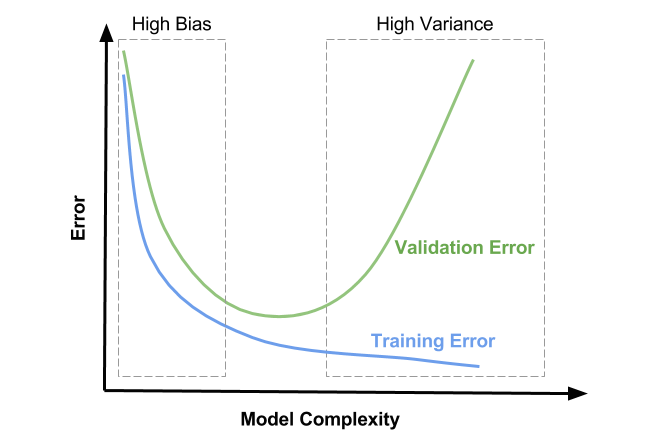
\includegraphics[width=0.65\linewidth]{images/18-error-plot.png}
	\caption{Visualisatie van training - en cross-validatiefout}
	\label{fig:error-plot}
\end{figure}

\subsection{\textit{Bias} en variantie regulariseren}

We kunnen ook de invloed van de regularisatieparameter $\lambda$ linken aan eventuele \textit{over -} of \textit{underfitting} van het model. Zoals we eerder al kort aangekaart hebben, is de functie van regularisatie het tegengaan van \textit{high variance}. Wanneer deze hyperparameter dus te klein is, hebben we te maken met \textit{overfitting} en wanneer $\lambda$ te groot is, hebben we te maken met \textit{underfitting}. Dit zien we op Figuur \ref{fig:error-plot-lambda}. 

\begin{figure}[h]
	\centering
	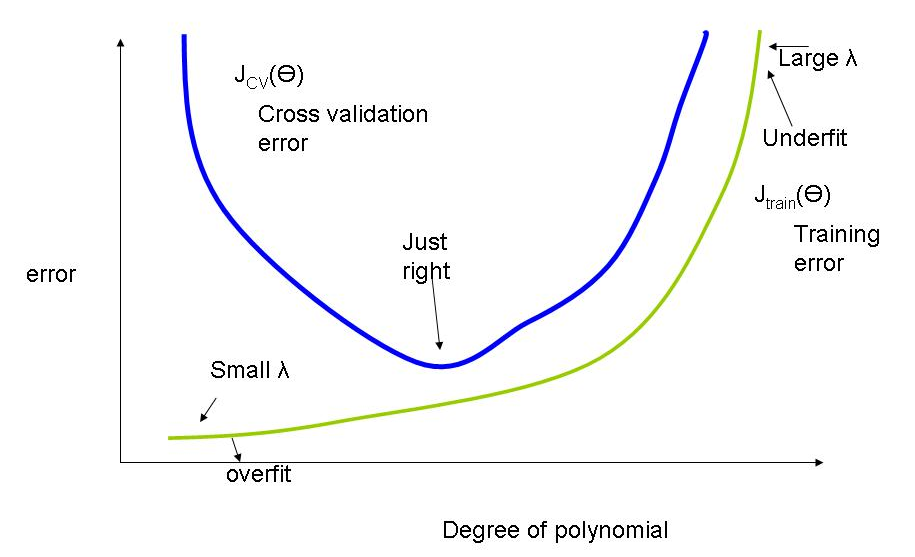
\includegraphics[width=0.65\linewidth]{images/19-error-plot-lambda.png}
	\caption{Visualisatie van training - en cross-validatiefout}
	\label{fig:error-plot-lambda}
\end{figure}
\noindent
We kunnen hier opnieuw een aantal modellen vergelijken, in dit geval allemaal getraind met een verschillende waarde voor de hyperparameter $\lambda$. Hierna zullen we op dezelfde manier de trainings - en crossvalidatiefout berekenen en op deze manier het meest geschikte model uitkiezen, namelijk die met de kleinste waarde voor $J_{CV}$. 

\subsection{Model selectie in neuraal netwerk}

Wanneer we kunnen kiezen uit een aantal  modellen met een verschillen aantal lagen en nodes, zullen we opnieuw de trainings - en cross-validatiefout berekenen en het model met de kleinste $J_{CV}$ kiezen. 

\subsection{Leercurves}

Leercurves (\textit{learning curves}) plotten de grootte van de trainings - en cross-validatiefout wanneer we de grootte van de training set doen toenemen. De groene curve op Figuur \ref{fig:learning-curves} stelt $J_{CV}$ voor en de blauwe curve is $J_{train}$. We zien dat $J_{train}$ toeneemt bij een toename van $m$, terwijl $J_{CV}$ afneemt. \\
\newline
In het geval van \textit{high bias}, zullen we een grote fout hebben op onze training - en cross-validatie set. Het toevoegen van extra trainingsdata zal hier niet helpen. Dit is bij \textit{high variance} wel het geval om de \textit{gap} tussen $J_{train}$ en $J_{CV}$ te doen afnemen.

\begin{figure}[h]
	\centering
	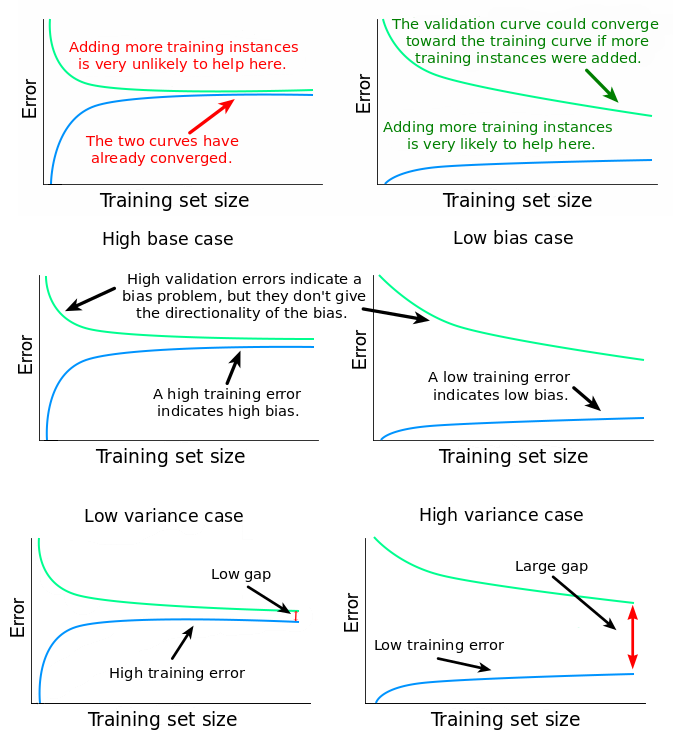
\includegraphics[width=0.5\linewidth]{images/20-learning-curves.png}
	\caption{Leercurves voor variantie en \textit{bias}}
	\label{fig:learning-curves}
\end{figure}
\newpage

\subsection{\textit{Bias} en variantie tegengaan}

We kunnen dus concluderen dat wanneer we te maken hebben met \textit{high bias}, we dit kunnen oplossen door extra \textit{features} toe te voegen, extra polynomiale \textit{features} toe te voegen of de regularisatieparameter $\lambda$ te verkleinen. \textit{High variance} kan tegengegaan worden door meer trainingsdata toe te voegen, minder \textit{features} te gebruiken of de regularisatieparameter $\lambda$ te vergroten. 

\subsection{K-fold cross-validatie}

Het doel achter K-fold cross-validatie is kijken hoe goed het model werkt op ongeziene data. Daarnaast dient het ook om omze hyperparameters te tunen. K-fold cross-validatie is een techniek die wordt toegepast op kleine datasets ($m < 10 000$). \\
\newline
De eerste stap van K-fold cross-validatie is het splitsen van onze dataset zoals op Figuur \ref{fig:kfold-step-1}. We zullen hier een splitsing maken in 80$\%$ voor de training set en 20$\%$ voor de test set. Dit splitsen van de dataset wordt ook wel \textit{data partitioning} genoemd. We kunnen nu zoals op Figuur \ref{fig:kfold-step-2}, 3 verschillende modellen gaan vergelijken met bijvoorbeeld elk een verschillend aantal lagen. Ter wijze van illustratie zullen we hiervoor 5 folds gebruiken. Dit betekent dat we onze trainingsdata in 5 gelijke delen opsplitsen. Hiervan zullen er telkens 4 als trainingsfold dienen en 1 als validatiefold. We kunnen dus 5 modellen bestuderen met telkens een andere validatiefold en andere trainingsfolds. Dit levert ons 5 verschillende performanties op, waarvan we het gemiddelde zullen berekenen. Dit is terug te zien op Figuur \ref{fig:kfold-folds}. Dit doen we voor elk van onze 3 mogelijke modellen. Op deze manier hebben we dus 15 modellen bestudeerd. We selecteren vervolgens het model dat de beste gemiddelde performantie oplevert. Dit wordt het model waarmee we verdergaan, zoals zichtbaar op Figuur \ref{fig:kfold-step-3}. Hierna zullen we het model testen met onze onafhankelijke testdata zodat we de performantie met deze data kunnen rapporteren (Figuur \ref{fig:kfold-step-4}). Ten slotte zouden we het bekomen model nog eens opnieuw kunnen trainen met de volledige dataset zoals op Figuur \ref{fig:kfold-step-5}. Dit is echter een optionele stap.
\newpage
\begin{figure}[h]
	\centering
	\begin{subfigure}{.70\textwidth}
		\centering
		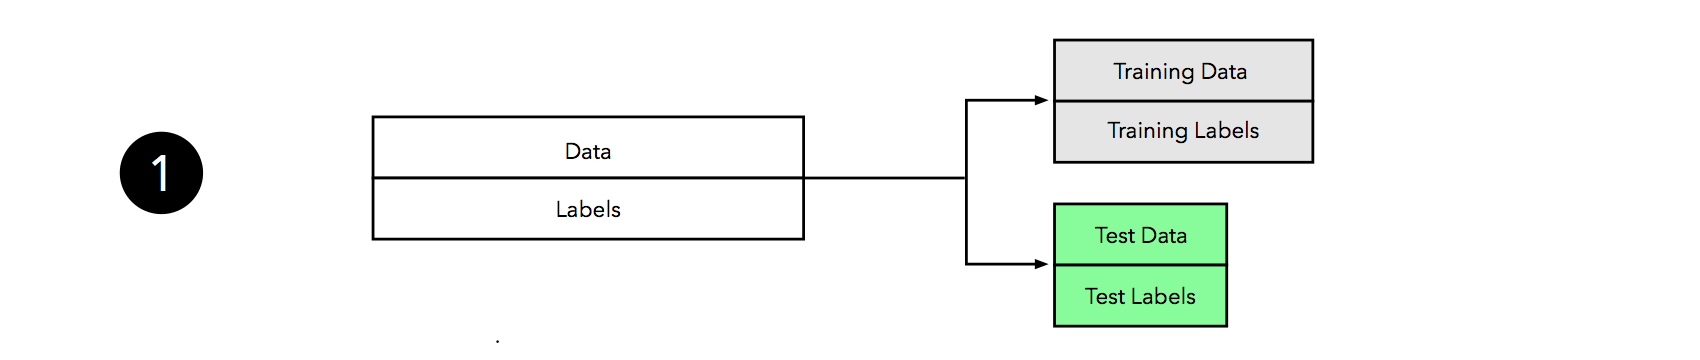
\includegraphics[width=\linewidth]{images/21-kfold-step-1.png}
		\caption{Stap 1 van K-fold cross-validatie}
		\label{fig:kfold-step-1}
	\end{subfigure}
	\begin{subfigure}{.70\textwidth}
		\centering
		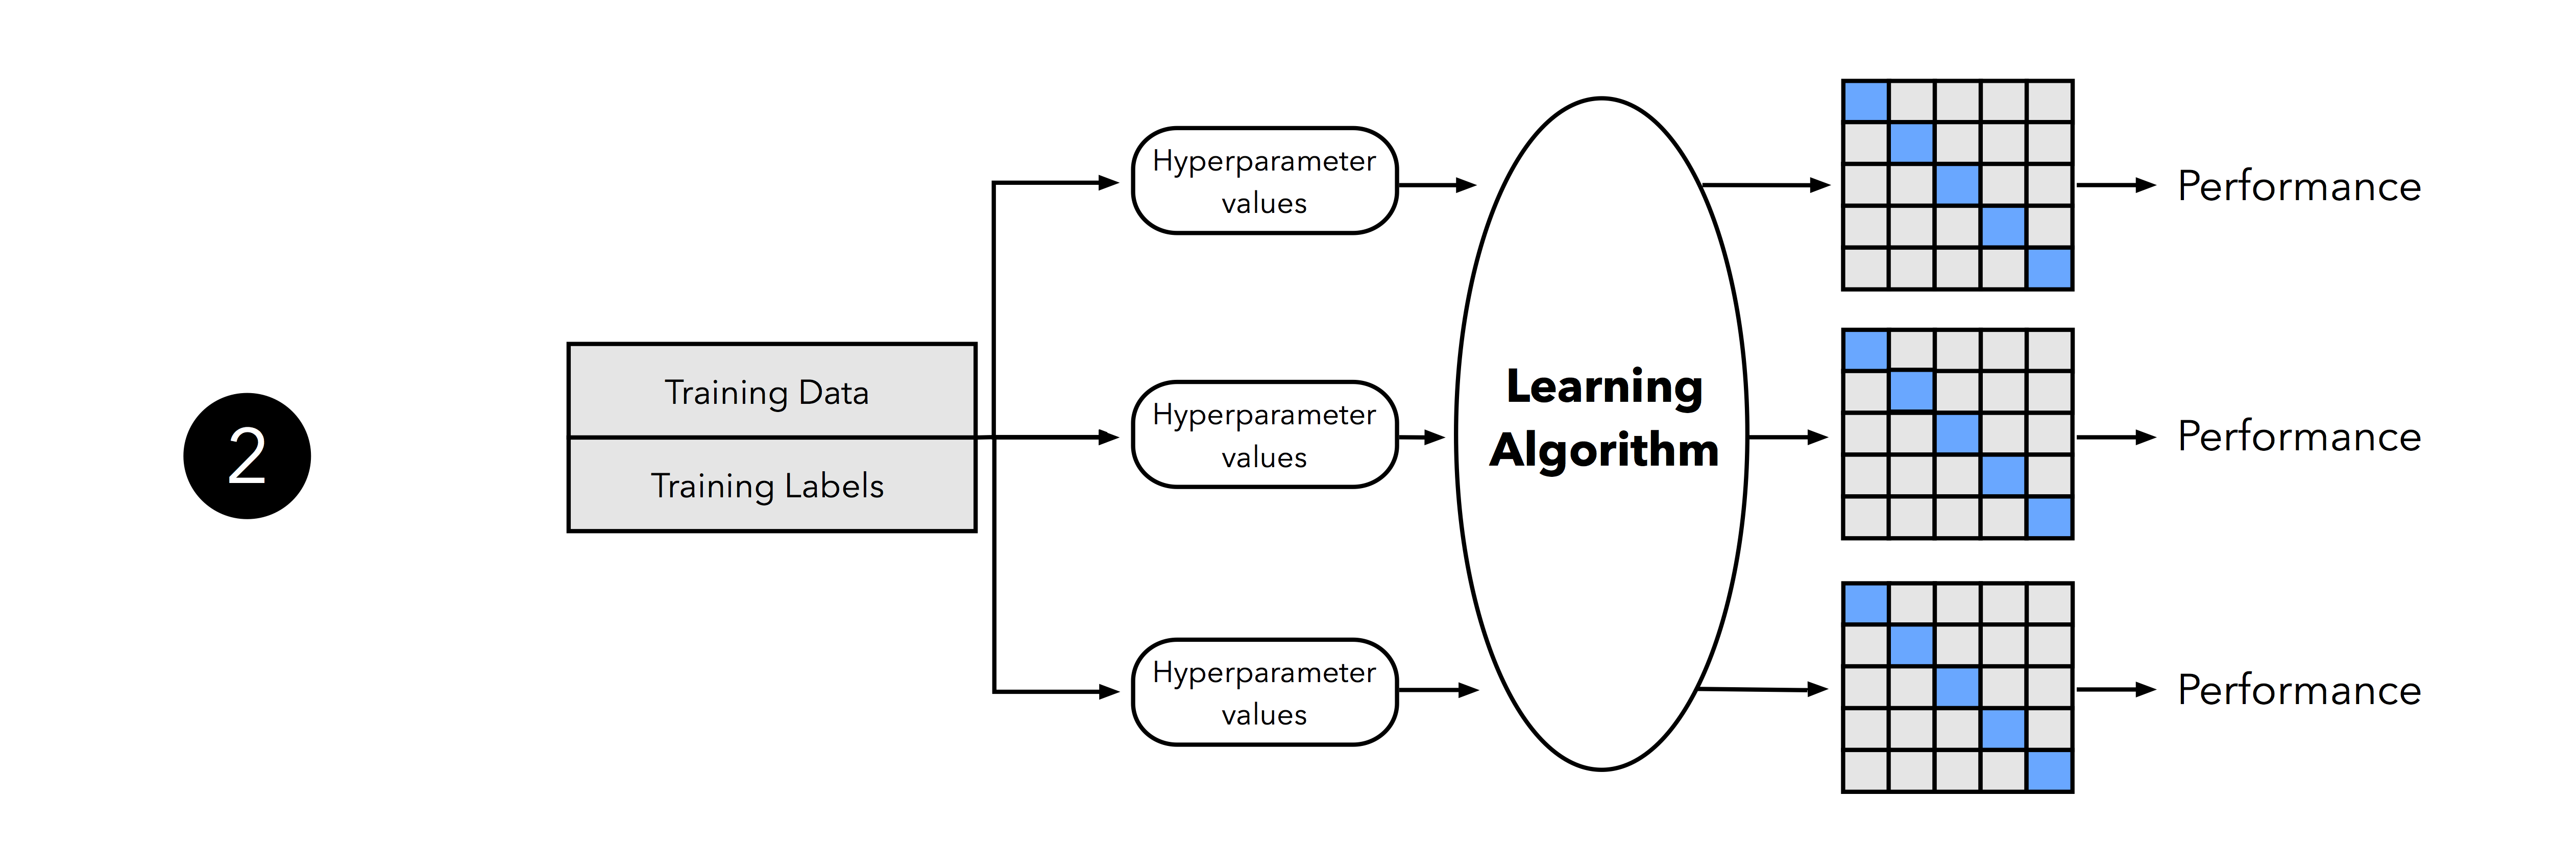
\includegraphics[width=\linewidth]{images/22-kfold-step-2.png}
		\caption{Stap 2 van K-fold cross-validatie}
		\label{fig:kfold-step-2}
	\end{subfigure}
	\begin{subfigure}{.5\textwidth}
		\centering
		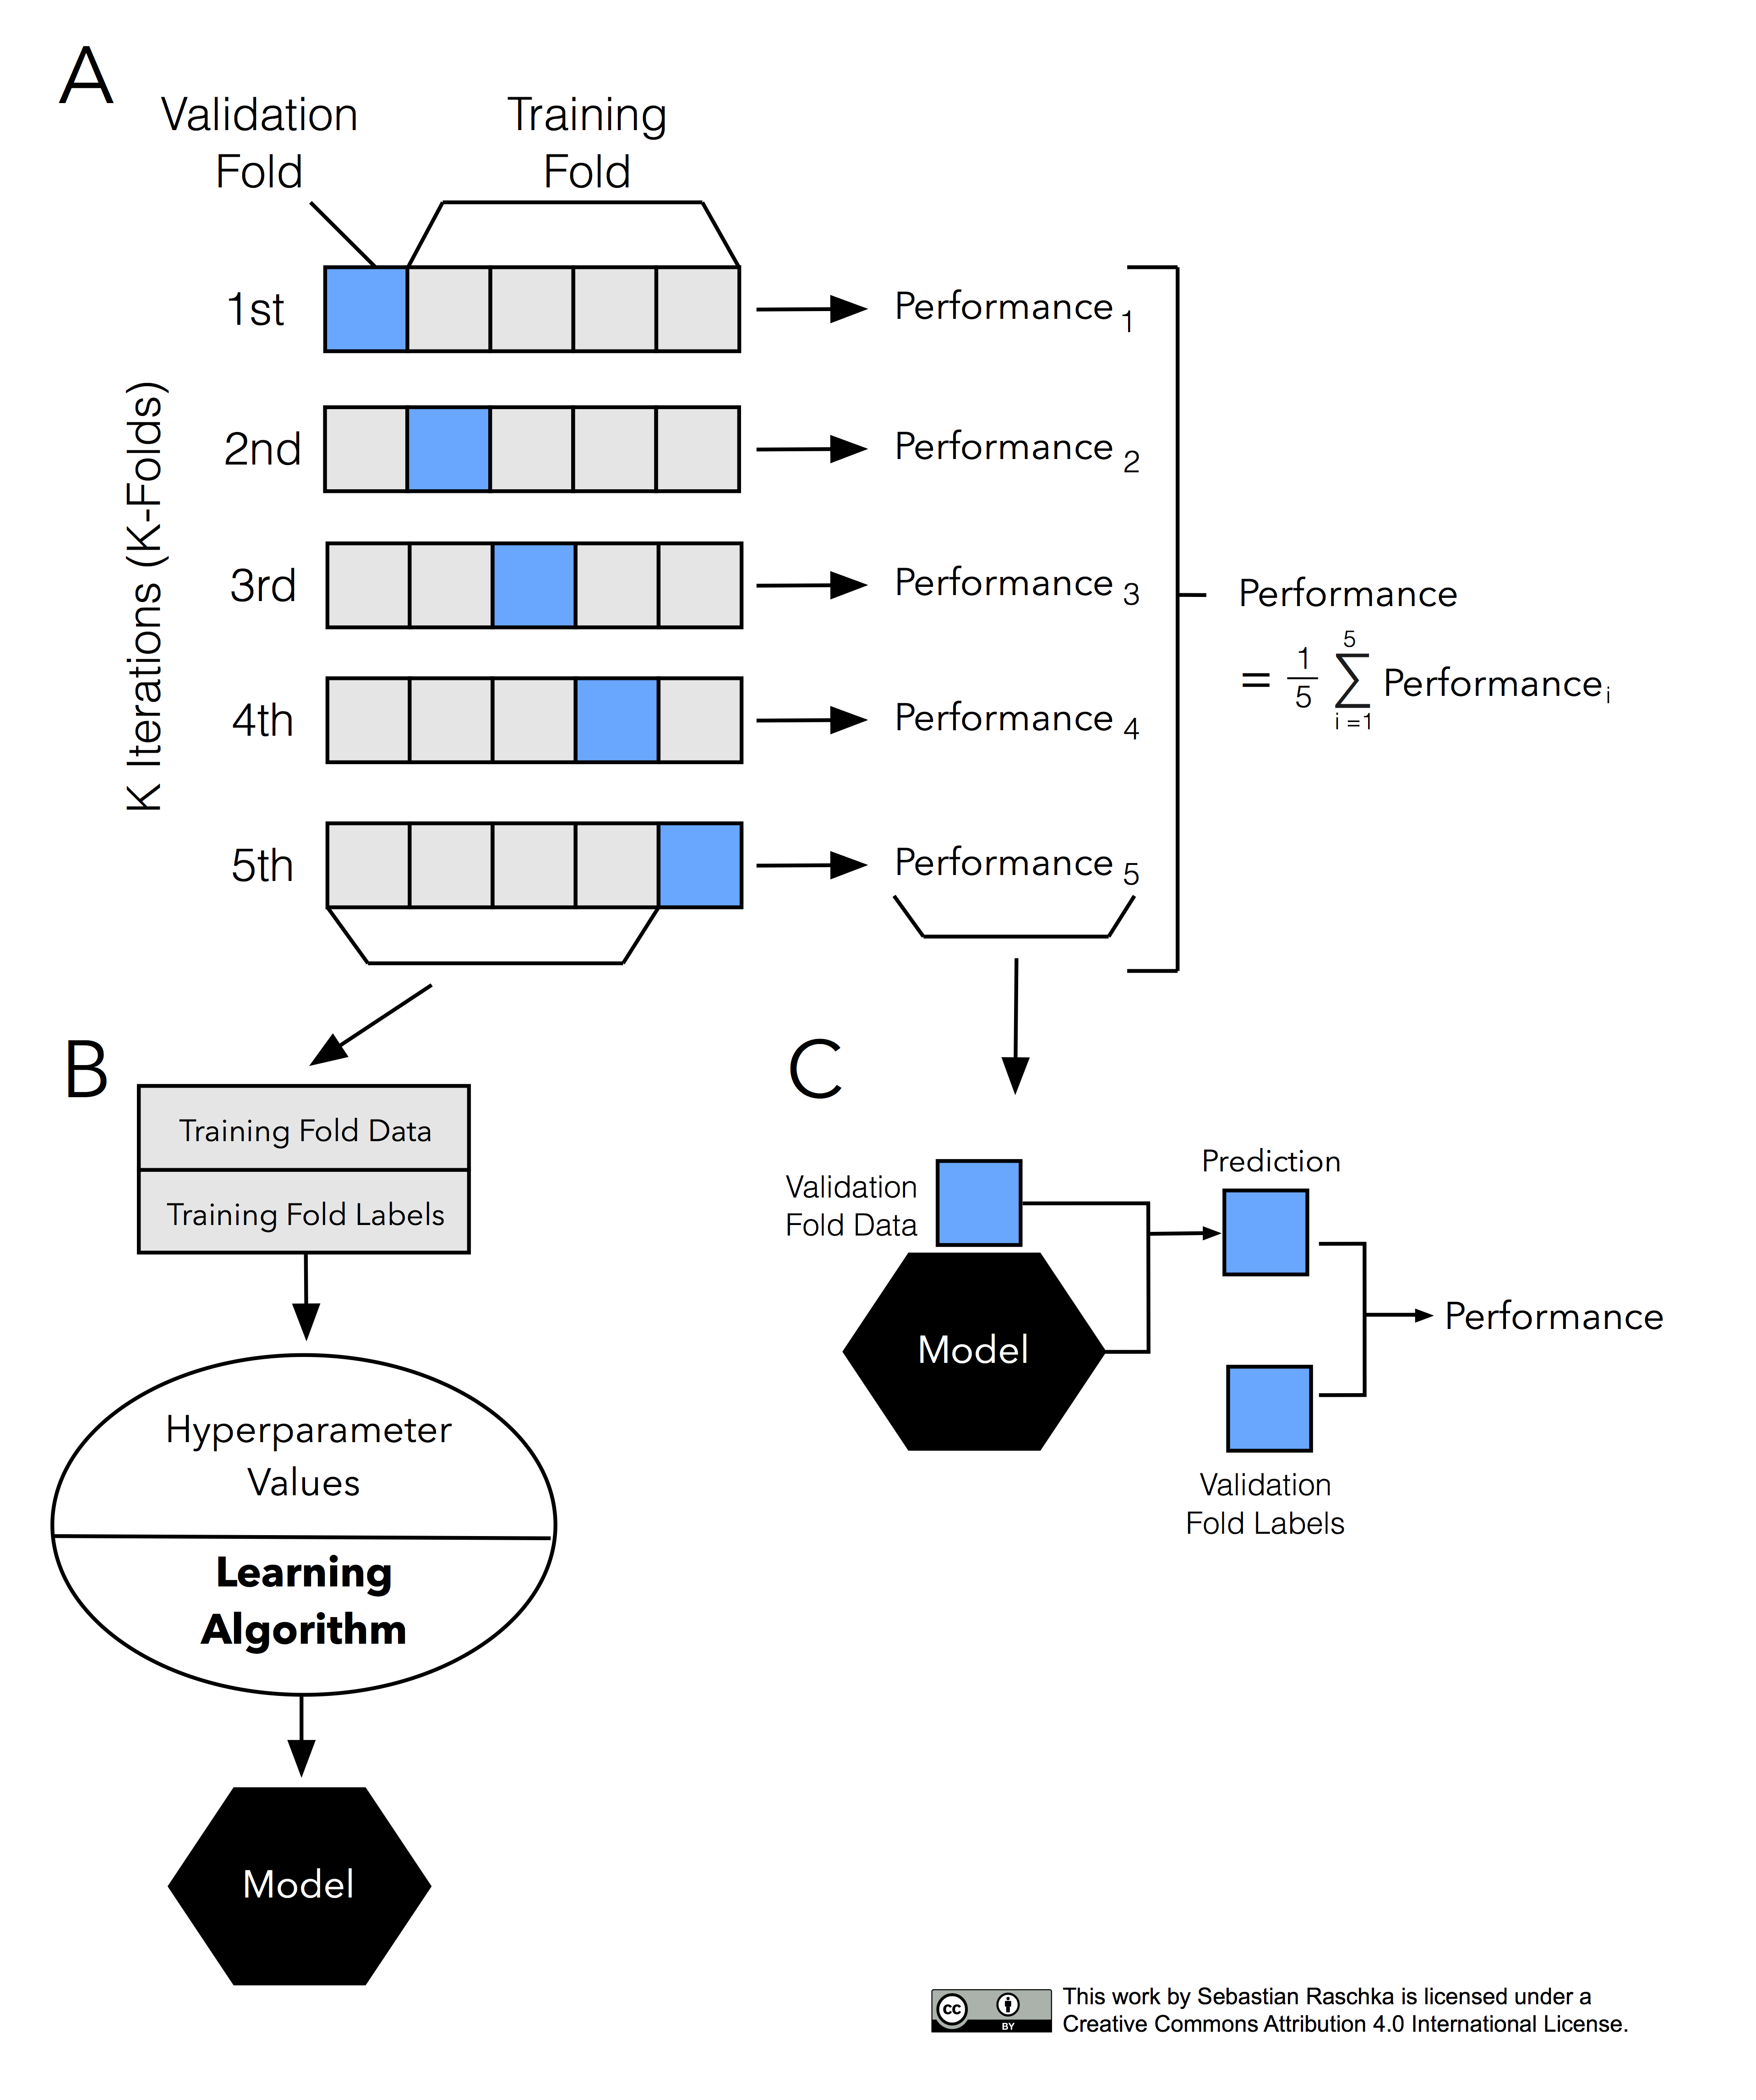
\includegraphics[width=\linewidth]{images/26-kfold-folds.png}
		\caption{Splitsing in training en validatie folds}
		\label{fig:kfold-folds}
	\end{subfigure}
	\caption{K-fold cross-validatie (deel 1)}
	\label{fig:kfold}
\end{figure}
\newpage
\begin{figure}[h]\ContinuedFloat
	\centering
	\begin{subfigure}{.70\textwidth}
		\centering
		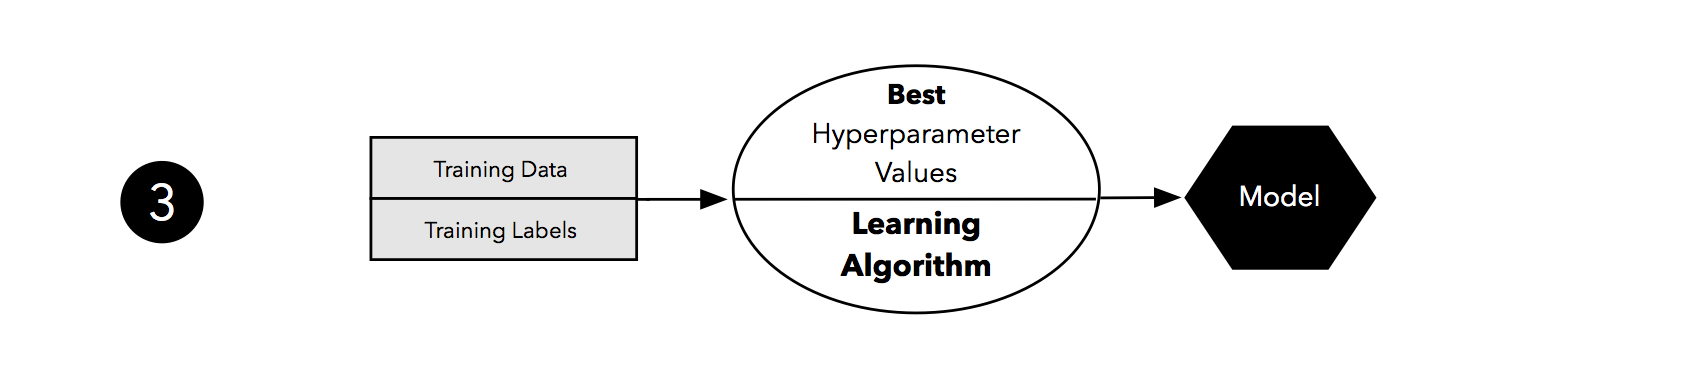
\includegraphics[width=\linewidth]{images/23-kfold-step-3.png}
		\caption{Stap 3 van K-fold cross-validatie}
		\label{fig:kfold-step-3}
	\end{subfigure}
	\begin{subfigure}{.70\textwidth}
		\centering
		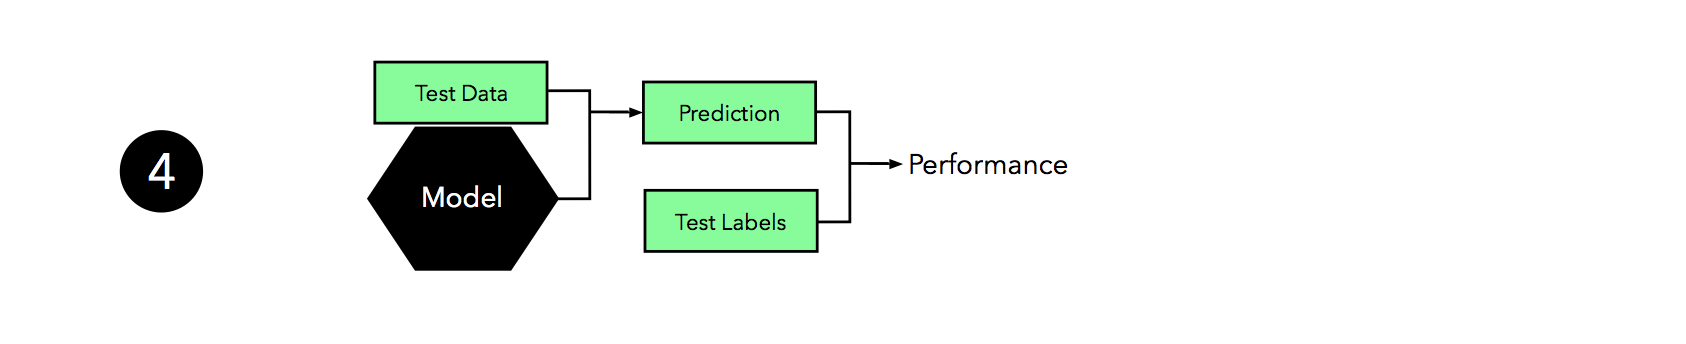
\includegraphics[width=\linewidth]{images/24-kfold-step-4.png}
		\caption{Stap 4 van K-fold cross-validatie}
		\label{fig:kfold-step-4}
	\end{subfigure}
	\begin{subfigure}{.70\textwidth}
		\centering
		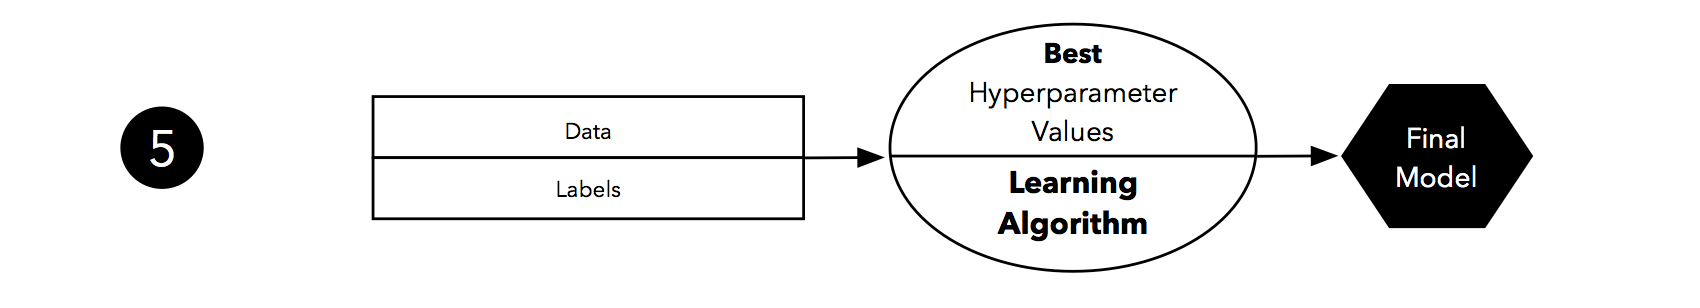
\includegraphics[width=\linewidth]{images/25-kfold-step-5.png}
		\caption{Stap 5 van K-fold cross-validatie}
		\label{fig:kfold-step-5}
	\end{subfigure}
	\caption{K-fold cross-validatie (deel 2)}
\end{figure}

\subsection{Error analyse}

Bij error analyse gaan we manueel de voorbeelden in onze cross-validatie set waar het model fouten op heeft gemaakt onderzoeken om zo te kijken of er een systematische trend in deze fouten zit. Als dit het geval is, kunnen we trachten dit op te lossen door het model meer te trainen op data waarop het fouten maakte.

\subsection{Confusion Matrix}
Een confusion matrix is een tabel die het aantal \textit{true positives}, \textit{true negatives}, \textit{false positives }en \textit{false negatives} weergeeft, zoals afgebeeld op Figuur \ref{fig:confusion-matrix}.

\begin{figure}[h]
	\centering
	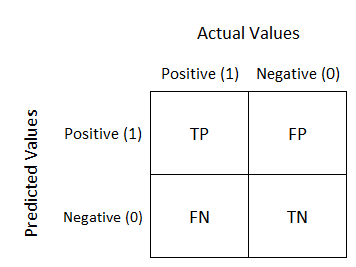
\includegraphics[width=0.4\linewidth]{images/27-confusion-matrix.png}
	\caption{Confusion Matrix voor binaire classificatie}
	\label{fig:confusion-matrix}
\end{figure}
\noindent
We kunnen de accuraatheid berekenen als:
\begin{equation}
	Acc = \frac{TP + TN}{TP + TN + FP + FN}
\end{equation}
\noindent
Dit levert ons een waarde tussen 0 en 1 op die we zo hoog mogelijk willen krijgen. \\
\newline
We kunnen op dezelfde manier een confusion matrix opstellen voor multi-class classificatie. Hierbij zal de accuraatheid opnieuw gelijk zijn aan het quotiënt van de som van alle \textit{true} labels en de som van alle predicties. Een belangrijke sidenote is wel dat accuraatheid enkel een goeie metriek is wanneer onze data gebalanceerd is. 

\subsection{Precision en recall}

De \textit{precision} en \textit{recall} zijn betere metrieken en worden als volgt berekend: 
\begin{equation}
	P  \frac{TP}{TP + FP}
\end{equation}
\begin{equation}
	R = \frac{TP}{TP + FN}
\end{equation}
\noindent
De \textit{precision} komt dus overeen met het aantal echte positieven ten opzichte van alle voorspelde positieven. Dit geeft dus weer hoeveel van de positieve voorspellingen effectief positief zijn. De \textit{recall} komt overeen met het aantal echte positieven ten opzichte van alle echte positieven. Dit geeft dus weer hoeveel van de echte positieven we correct voorspeld hebben. Beide maten geven ons een waarde tussen 0 en 1 die we zo hoog mogelijk willen krijgen. De \textit{true negatives} worden in beide metrieken niet meegerekend. \\
\newline
We moeten een afweging maken tussen \textit{precision} en \textit{recall}. Figuur \ref{fig:precision-recall} stelt dit grafisch voor. Stel je voor dat we een logistisch regressieprobleem hebben. Wanneer we met grote zekerheid $y=1$ willen voorspellen  (en dus de drempelwaarde verhogen), zal de \textit{precision} toenemen, maar de \textit{recall} afnemen. Omgekeerd, als we willen vermijden dat we te veel positieven missen (en dus de drempelwaarde verlagen), zal de \textit{precision} afnemen, maar de \textit{recall} toenemen. De \textit{sweet spot} die we zouden willen bereiken is daar waar zowel de \textit{precision} als de \textit{recall} gelijk zijn aan 1.

\begin{figure}[h]
	\centering
	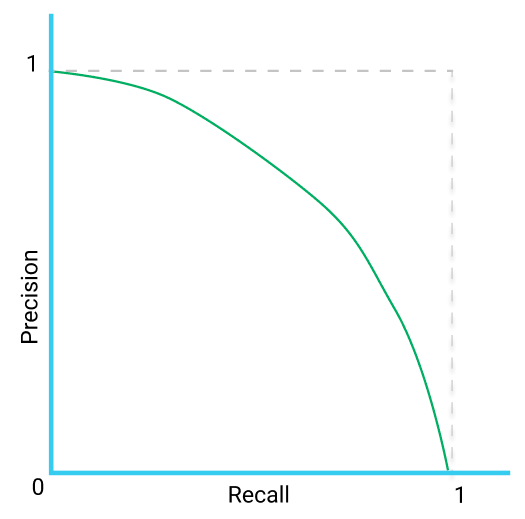
\includegraphics[width=0.4\linewidth]{images/28-precision-recall.png}
	\caption{Afweging tussen \textit{precision} en \textit{recall}}
	\label{fig:precision-recall}
\end{figure}

\subsection{F1 score}

Het is moeilijk om de \textit{precision} en \textit{recall} te vergelijken. Wanneer we zouden proberen om het gemiddelde te nemen om beiden te vergelijken, merken we dat ongebalanceerde data een vertekend beeld geeft. Daarom is de F1 score uitgevonden om beide metrieken te vergelijken. Deze wordt als volgt berekend:
\begin{equation}
	F1 = 2\frac{P\cdot R}{P +R}
\end{equation}
\noindent
Dit zal opnieuw een waarde tussen 0 en 1 opleveren.

\subsection{Toevoeging van extra data}

Het is niet altijd mogelijk om nieuwe data toe te voegen. Daarom gaan we onze bestaande data modificeren om deze als extra data te gebruiken. Wanneer we bijvoorbeeld een model trainen met afbeeldingen van katten, kunnen we een bestaande foto een beetje scheef zetten of inzoomen om deze zo als nieuwe data te gebruiken. \\
\newline
Wanneer we onze performantie bestuderen in functie van onze hoeveelheid beschikbare data, zullen we zien dat deze altijd zal toenemen naarmate we meer data beschikbaar hebben en meer lagen kunnen toevoegen aan ons model. Daarom is er meer en meer een verschuiving aan het plaatsvinden van een conventionele model-centrische aanpak naar een data-centrische aanpak, waarbij we eerder focussen op onze hoeveelheid data dan op ons model zelf.

\subsection{Transfer learning}

Bij transfer learning gaan we starten vanaf een op voorhand getraind model dat getraind is op een grote dataset met hetzelfde input type als onze applicatie, en vervolgens dit model verder trainen met onze eigen data.
